\section{Method of Characteristics}
\label{sec:characteristics}

This section derives an implicit solution formula for the inviscid
Burgers' equation via the method of characteristics. The formula's
eventual breakdown is what forces the more general framework of
Sections~\ref{sec:shock-formation}--\ref{sec:entropy-condition}.

\subsection{Setup}
\label{subsec:char-setup}

Consider the initial value problem
\begin{equation}
  \label{eq:ivp}
  \begin{cases}
    u_t + u\, u_x = 0, & x \in \mathbb{R},\ t > 0, \\
    u(x,0) = u_0(x), & x \in \mathbb{R},
  \end{cases}
\end{equation}
with $u_0 \in C^1(\mathbb{R})$. The method of characteristics looks for
curves $x(t)$ along which the PDE reduces to an ODE for $u(x(t),t)$.

\subsection{Derivation of the characteristic equations}
\label{subsec:char-derivation}

For a solution $u$ of \eqref{eq:ivp} and a curve $x(t)$, the chain rule
gives
\begin{equation}
  \label{eq:chain-rule}
  \frac{d}{dt}\, u(x(t), t) = u_x(x(t),t)\, \dot{x}(t) + u_t(x(t),t).
\end{equation}
Since $u_t = -u\,u_x$ on solutions, choosing $x(t)$ to satisfy
\begin{equation}
  \label{eq:char-ode-x}
  \dot{x}(t) = u(x(t), t)
\end{equation}
reduces \eqref{eq:chain-rule} to
\begin{equation}
  \label{eq:char-ode-u}
  \frac{d}{dt}\, u(x(t), t) = 0.
\end{equation}
Curves satisfying \eqref{eq:char-ode-x} are \emph{characteristics}, and
$u$ is constant along each one.

\subsection{Characteristics are straight lines}
\label{subsec:char-lines}

\begin{proposition}[Characteristics are straight lines]
\label{prop:char-lines}
Let $u$ be a $C^1$ solution of \eqref{eq:ivp} on $\mathbb{R} \times
[0,T)$, and let $x(t)$ solve \eqref{eq:char-ode-x} with $x(0)=x_0$. Then
for $0 \le t < T$,
\begin{equation}
  \label{eq:char-formula}
  u(x(t), t) = u_0(x_0), \qquad x(t) = x_0 + u_0(x_0)\, t.
\end{equation}
\end{proposition}

\begin{proof}
By \eqref{eq:char-ode-u}, $u(x(t),t) \equiv u(x_0,0) = u_0(x_0)$.
Substituting this constant into \eqref{eq:char-ode-x} gives $\dot x(t) =
u_0(x_0)$, which integrates to the stated formula for $x(t)$.
\end{proof}

Thus any classical solution is completely determined by
\eqref{eq:char-formula}, reducing its construction to inverting $x_0
\mapsto x = x_0 + u_0(x_0)\, t$ at each fixed $t$.

\subsection{The implicit solution formula}
\label{subsec:char-implicit-formula}

\begin{theorem}[Implicit solution via characteristics]
\label{thm:implicit-solution}
Let $u_0 \in C^1(\mathbb{R})$. For each $t \geq 0$ such that $\Phi_t :
\mathbb{R} \to \mathbb{R}$, $\Phi_t(x_0) = x_0 + u_0(x_0)\, t$, is a
bijection with $C^1$ inverse, the function $u$ defined implicitly by
\begin{equation}
  \label{eq:implicit-solution}
  u(x,t) = u_0(x_0), \qquad \text{where } x = x_0 + u_0(x_0)\, t,
\end{equation}
is the unique $C^1$ solution of \eqref{eq:ivp} at time $t$.
\end{theorem}

\begin{proof}
\emph{Well-definedness.} Bijectivity of $\Phi_t$ means $u(x,t) =
u_0(\Phi_t^{-1}(x))$ is well defined, and $C^1$ since $\Phi_t^{-1}$ and
$u_0$ are.

\emph{The PDE holds.} Write $x_0 = x_0(x,t) = \Phi_t^{-1}(x)$.
Differentiating $x = x_0 + u_0(x_0)\, t$ in $x$ and in $t$ gives
\begin{equation}
  \frac{\partial x_0}{\partial x} = \frac{1}{1 + u_0'(x_0)\,t},
  \qquad
  \frac{\partial x_0}{\partial t} = \frac{-u_0(x_0)}{1 + u_0'(x_0)\, t},
\end{equation}
both well defined since $\Phi_t'(x_0) = 1+u_0'(x_0)t \neq 0$. By the chain
rule applied to $u(x,t) = u_0(x_0(x,t))$,
\begin{equation}
  u_x = \frac{u_0'(x_0)}{1 + u_0'(x_0)\,t},
  \qquad
  u_t = \frac{-u_0(x_0)\, u_0'(x_0)}{1 + u_0'(x_0)\, t},
\end{equation}
so $u_t + u\,u_x = 0$, and $u(x,0)=u_0(x)$ since $\Phi_0=\mathrm{id}$.

\emph{Uniqueness.} Any $C^1$ solution must, by
Proposition~\ref{prop:char-lines}, agree with \eqref{eq:implicit-solution}
along every characteristic.
\end{proof}

\begin{corollary}[Local existence]
\label{cor:local-existence}
For $u_0 \in C^1(\mathbb{R})$ with $u_0'$ bounded below, there exists
$T>0$ such that \eqref{eq:ivp} has a unique $C^1$ solution on $\mathbb{R}
\times [0,T)$, given by \eqref{eq:implicit-solution}.
\end{corollary}

\begin{proof}[Proof sketch]
It suffices that $\Phi_t'(x_0) = 1+u_0'(x_0)t$ stay bounded away from $0$
uniformly in $x_0$ for $t \in [0,T)$; monotonicity of $\Phi_t$ then gives
bijectivity with $C^1$ inverse. Let $m = \inf_{x_0} u_0'(x_0)$. If $m \geq
0$, then $\Phi_t'(x_0) \geq 1$ for all $t\geq0$ and $T=\infty$ works. If
$m<0$, then $\Phi_t'(x_0) \geq 1+mt > 0$ for $t < -1/m$, so any $T \leq
-1/m$ works.
\end{proof}

The bound $T \leq -1/m$ is not an artefact of the proof: it is the exact
breakdown time, as Proposition~\ref{prop:shock-time} shows.

\subsection{Worked example}
\label{subsec:char-example}

Let $u_0(x) = -\arctan(x)$, so $u_0'(x) = -1/(1+x^2) \in [-1,0)$. By
Theorem~\ref{thm:implicit-solution}, the solution satisfies
\begin{equation}
  u(x,t) = -\arctan(x_0), \qquad x = x_0 - \arctan(x_0)\, t,
\end{equation}
valid while $\Phi_t'(x_0) = 1 - t/(1+x_0^2) > 0$ for all $x_0$. Since
$1/(1+x_0^2)$ is maximised at $x_0=0$, this holds exactly for $t<1$: the
characteristic through the origin, carrying the steepest slope
$u_0'(0)=-1$, is the first to cause $\Phi_t$ to fail to be injective, at
$t=1$.

\begin{figure}[h]
\centering
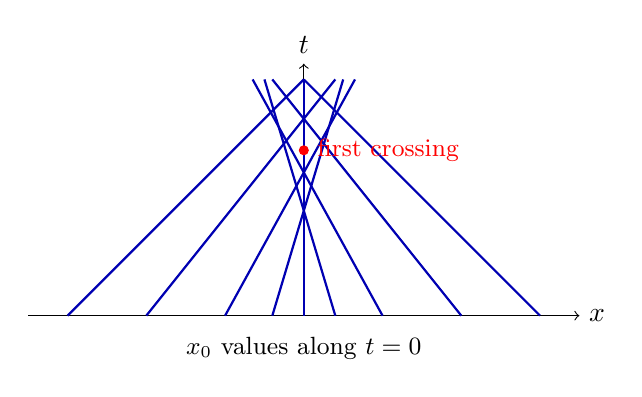
\begin{tikzpicture}[scale=1.0]
  \draw[->] (-3.5,0) -- (3.5,0) node[right] {$x$};
  \draw[->] (0,0) -- (0,3.2) node[above] {$t$};
  \foreach \xz/\slope in {-3/1.0, -2/0.8, -1/0.55, -0.4/0.3, 0/0, 0.4/-0.3, 1/-0.55, 2/-0.8, 3/-1.0}{
    \draw[thick, blue!70!black] (\xz,0) -- ({\xz+\slope*3},3);
  }
  \filldraw[red] (0,2.1) circle (1.6pt);
  \node[red, right] at (0.05,2.1) {\small first crossing};
  \node[below] at (0,-0.15) {\small $x_0$ values along $t=0$};
\end{tikzpicture}
\caption{Characteristics for decreasing initial data $u_0$. Where $u_0$
is decreasing, characteristics converge; the first crossing time is
$T=-1/\min u_0'$ (Corollary~\ref{cor:local-existence}), computed
precisely in Section~\ref{sec:shock-formation}.}
\label{fig:characteristics}
\end{figure}

\begin{remark}[What happens beyond $T$]
\label{rem:beyond-T}
Once two characteristics carrying different values of $u_0$ meet, formula
\eqref{eq:implicit-solution} assigns $u$ two values at once, so no
single-valued classical solution can exist beyond this time. Making sense
of the equation past this point is the subject of
Sections~\ref{sec:shock-formation} and \ref{sec:weak-solutions}.
\end{remark}